\documentclass[11pt]{article}
\usepackage{multicol,graphicx,float}
\usepackage[margin=1 in]{geometry}
\title{An Extension of Two-Dimensional Detection Function Distance Sampling Software}
\date{January 2017}
\author{Calliste Fagard-Jenkin}

\begin{document}
\pagenumbering{gobble}
\maketitle
\begin{center}

\includegraphics[scale=1]{Logo}
\end{center}
\newpage
\begin{multicols}{2}
\pagenumbering{arabic}	
	
\section{Introduction}
\subsection{Context and background}
\subsubsection{Initial overview}
This project focuses on line-transect distance sampling; a hybrid method which uses both design and model based inference to produce estimates on the sizes of animal populations. An extension of distance sampling by Borchers and Cox (2017) allows for the use of 2D detection functions, describing the probability of detection of an animal in both forward and perpendicular directions. This methodology produces estimates of abundance which are far less biased when compared to estimates produced by conventional distance sampling, when the animals in the population of interest display responsive movement. The raison d'etre of this project is to further extend the code-base of the Borchers and Cox (2017) methodology's R package (called LT2D) and to provide a number of illustrative analyses on a range of datasets to demonstrate the improved functionality.

\subsubsection{What is distance sampling?}

Distance sampling is a methodology within ecological statistics which allows us to produce unbiased estimates of animal population sizes even when the detection of any individual in the survey area is uncertain. First, a quick description of its simpler younger brother, strip sampling (in which detection of individuals is certain), will be given in order to illustrate the fundamental principles of greatest importance. 

Consider a survey area within which the population of interest is closed (there is no emigration or immigration of individuals). We further assume that births and deaths are considered to occur at a negligible rate. In this way, the survey is considered to be a snapshot of the population at some given moment. In our example, we choose a square survey area, which we subdivide into five strips of regular width. Animals are uniformly distributed throughout the survey area, in both the perpendicular and the horizontal axis. This is illustrated by figure 1. 

\begin{figure}[H]
\centering
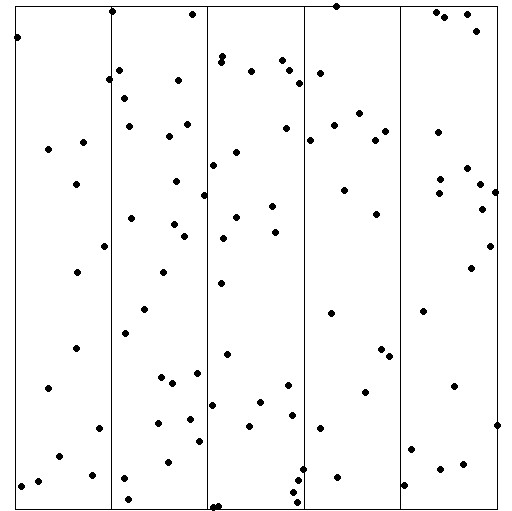
\includegraphics[scale=0.5]{StripSampling}
\caption{Example distribution of animals in a square survey area divided into 5 equal strips}
\end{figure}

Given this rather simplistic design, obtaining an estimate of abundance in the survey area ($\hat{N}$) is extremely simple, so long as we are able to sample all of the individuals within whole strips. As an example we consider strips 2 and 4 (from the left) as the randomly selected strips which form our survey sample. Strip 2 contains 25 individuals, and strip 4 contains 15, giving us a total of $n=40$ observed individuals. If we denote the total survey area by $A$ and the sampled area by $a$, then we observe that our survey effort of $\frac{a}{A}=\frac{2}{5}$. Hence a reasonable intuitive estimator for the abundance in the whole survey area is
\begin{equation}
\hat{N}=\frac{n}{\frac{a}{A}}=\frac{40}{0.4}=100
\end{equation}
which is a simply a rescaling of the number of observed animals which accounts for the portion of the survey area which has remained unseen. This example forms a basic overview of an easy methodology we can use when detection of every individual is guaranteed, however, we would now like to find a way of relaxing this rather unrealistic assumption. If we assume all animals in the strip have some fixed probability $p$ of being detected, then we can modify our estimator to account for the animals we expect we have missed:
\begin{equation}
\hat{N}=\frac{n}{\frac{a}{A}p}
\end{equation} 
This again is nothing more than rescaling the estimate by an appropriate constant. 

The real hard work begins when we start to ask ourselves how we can estimate this value of average detection probability, which turns out not to be so simple. However, distance sampling comes to the rescue!  In line transect distance sampling, one or multiple observers travel along a transect line which has been pre-determined by the experimental design. Observers look to the left and right of the line as they travel along its path (either on foot, by plane, boat, car etc) and record the perpendicular distance at which each observed animal was detected at. Once we pool together all these perpendicular distances for all detected animals, we expect to see a histogram similar to figure 2, which clearly displays that the frequency of detection drops as perpendicular distance increases. This trend has a rather obvious explanation, owing to the fact that animals become harder and harder to see the farther away they are.

\begin{figure}[H]
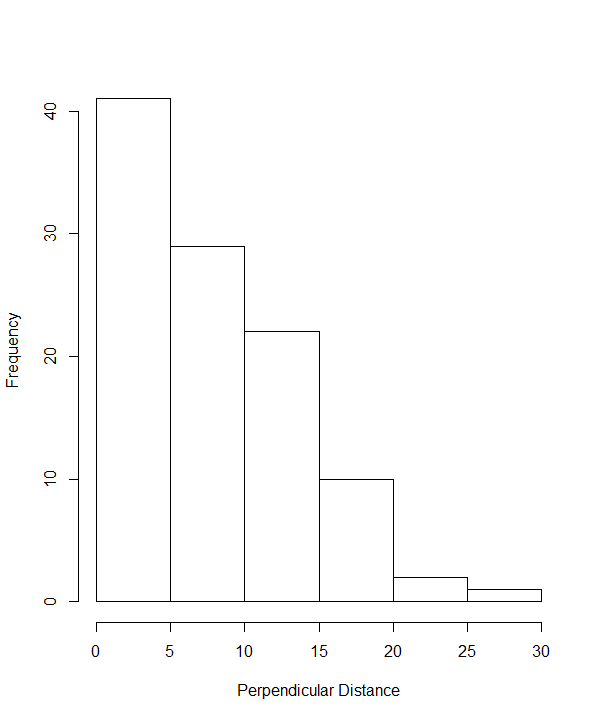
\includegraphics[scale=0.5]{DistanceHist}
\caption{Histogram of perpendicular distances of detected animals}
\end{figure}

A model-based approach which involves the fitting of a detection function, allows us to estimate the way in which distance affects detection probability. Figure 3 illustrates this by overlaying a (scaled) half-normal detection function over simulated detection data. Over the course of an analysis, multiple detection functions will be fitted to the data and the most appropriate one selected. In the case of the Distance package written and maintained by the Centre for Research into Ecological and Environmental Modelling, Saint Andrews, this is done by the numerical computation of maximum likelihood estimates.

\begin{figure}[H]
\centering
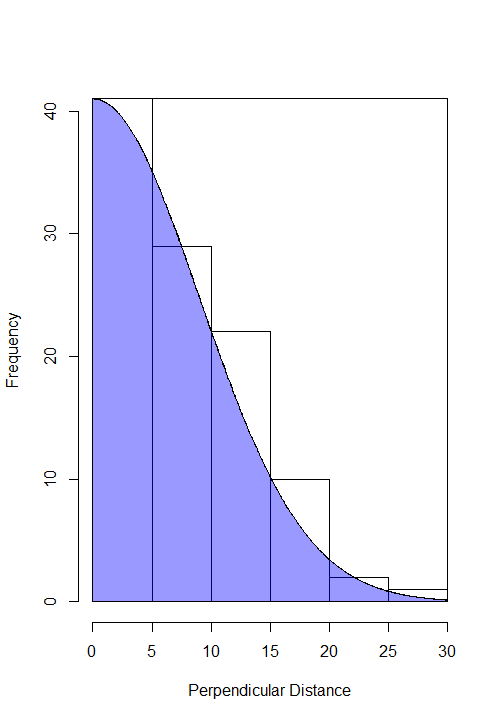
\includegraphics[width=6.38cm]{DistHistDetec}
\caption{Histogram of detection distances with overlayed detection function}
\end{figure}

If we momentarily return to the case of perfect detection, we notice that we would expect to see a perfectly flat histogram of perpendicular detection distances (as a result of uniform distribution of animals about the transect line). In this case the bars of our histogram would perfectly cover both the shaded, and un-shaded areas of Figure 3. Hence, the ratio of our detections with respect to this 'perfect detection rectangle' gives us some indication of the average detection probability of the population of interest. In practice, the 'perfect area rectangle' is extremely easy to calculate, and the area covered by our own detections is seen as the integral of the detection function over an interval from $0$ to a chosen perpendicular truncation distance $w$. In order to obtain the sampled area ($a$, in the previous example) in the case of a line transect distance sampling survey, we simply consider $a=2Lw$, where $L$ is the total length of all covered transect lines and $w$ is the previously mentioned perpendicular truncation distance. Thus, with these tools at our disposal, we can modify (2) to obtain:
\begin{equation}
\hat{N}=\frac{n}{\frac{2Lw}{A}\hat{p}}
\end{equation}
where $\hat{p}$ is the estimate of average detection probability we obtain by integrating the detection function and considering the area of the 'perfect detection rectangle'. It should be noted that this description of distance sampling is extremely rudimentary, and is far more intuitive than it is technical. For a deeper understanding of the likelihood functions involved, the design-based, and model-based aspects of the method, reference should be made to classic literature, such as Buckland, et al. 2015 and Borchers, et al. 2002. 

\subsubsection{The significance of 2D detection functions}

One of the assumptions of distance sampling is that the distribution of animals about the transect line is known. In the previous case of line-transects, it was uniform (however in point transect distance sampling it is typically triangular). Unfortunately, there are many situations in which this assumption is strongly violated, leading to significant bias in estimates of animal abundance and density. One reason for this could be poor survey design, whereby insufficient randomisation of transect line locations leads to trends in the distribution of animals between them. There is no effective analytical solution for poor survey design, and so this case is not considered here. A more interesting cause for this phenomenon is responsive movement of animals in the population of interest. Animals can be scared by observers and hence move away, causing a dip in observed detection frequencies on and close to the transect line, as well a spike in observed detection frequency some relatively small distance away from the transect line. This behaviour is typically referred to as avoidance, and is extremely common in primates, with gibbons being so notoriously prone to the behaviour that they are the subject of regular conventions between ecologists and statisticians, and thus they will be used as one of the illustrative case studies within this project. Conversely, animals may also display attraction, whereby an attraction to the transect line cause a spike in detections on the transect line and a dip further out, dolphins typically display this behaviour when data is collected via shipboard surveys, where the wake of the vessel draws them in.
\subsection{Previous contributions}

From June - August 2017 I undertook work on the code-base as a summer student. The notable changes I made to this code-base over this period will be clearly outlined in this section to distinguish them from the work which was undertaken from September 2017 onward as part of this project, however these will be not be described in depth, in order to avoid removing any focus from the improvements made as a part of this project. If more detail on the work conducted in this summer studentship is of interest, it can be found in the slides of a presentation conducted at the 2017 St Andrews Mathematics Undergraduate Research Conference, which have been included in the appendix. 

\subsubsection{Object Oriented Additions}
The R programming language allows for packages to include their own classes to produce objects with behaviours and properties tailored to the task at hand. These typically come in the form of S3 or S4 objects. As part of my summer work I wrote methods for S3 generic functions which allow the LT2D package to be more streamlined and provide the user with a cleaner and more straight forward interface with the functionality provided under the hood. The first set of these methods are dedicated to the R plot function, allowing the user to plot LT2D fitted model objects with a simple call to the generic plot function, with the aforementioned object as the first argument. 

\subsubsection{Adding in Abundance Estimation}
Previous versions of the code-base only produced estimates for average detection probability, $\hat{p}$. Code supplied by Prof. Borchers was modified and integrated with existing LT2D code to allow the package to produce estimates of abundance as well as average detection probability. This work was done towards the end of the project and hence was not fully integrated and tested with all other pieces of functionality available within the software, therefore modifications of abundance estimation code and its continual testing and iterative improvement is necessary for the completion of this project, however the details of these updates are of far less interest than the more ambitious aspects of the project and so they shall not be mentioned further in any significant amount of detail. Any addition or modification of code or theoretical technicalities related to the LT2D package mentioned out-with of section 1.2 are not a result of previous work and form the improvements and extensions which the project aims to produce.

\subsubsection{Rounded Angles}
When measurements of small detection angles are rounded down to $0$ in the field, the magnitude of the bias of estimated average detection probability, $\hat{p}$, can drastically increase. An appropriate modification to the method's likelihood function was theorised by prof. Borchers and then I implemented the new functionality into the source code. I conducted multiple simulations to confirm that bias was significantly reduced, all of which clearly demonstrated the new estimator performed far better.

\subsubsection{New Perpendicular Density}
A reparameterization of an existing perpendicular density was required to allow for a  half-normal perpendicular density function with a non-zero expected quantity of animals on the transect line. Prof. Borchers and I decided on a suitable formulation and I implemented it within the LT2D package. 

\subsubsection{Concatenation of GoF functions}
Goodness of fit tests (Cramer Von Mises and Kolmogorov-Smirnov) are conducted separately in the x and y (perpendicular and forward) directions, respectively, by the LT2D. These were split into distinct functions, making their use tedious to the end user. I rectified this issue by creating a wrapper function which was easier for the user to interact with and acted as an interface with the pre-existing code.

\subsubsection{Model Collecting and Summarising}
As with many model-based statistical methodologies, it is often good practice to fit a range of varied models to the available data, and to use selection criteria (such as Akaike's Information Criterion) to select which model(s) are most reasonable. This leads to the user's R global environment being peppered with objects created by the LT2D package, making it difficult to keep track of the models of interest. Inspired by another piece of software used for animal abundance (RMARK - An interface to the popular MARK windows software used as a tool for analysis of mark-recapture data), model-collecting and comparison-table-generating functions were implemented within the LT2D package.

\subsection{Project objectives and outline}
The project aims to include the ability for users to specify covariate inclusion for the two-dimensional detection functions, making them not only a function of perpendicular and forward distance, but also of user-defined relationships between other variables. Upon discussion with Prof. Borchers, it was decided this functionality should be kept as general as possible, following the following main criteria:

\begin{enumerate}
\item Users should be able to choose whether the covariate affects the behaviour of the detection function in the perpendicular direction, the forward direction or at the intercept, or any combination of the above.
\item Users should be able to define the formula which describes the linear predictor for the relevant parameter and the covariate(s) of interest themselves, rather than be restricted to pre-defined options
\item Users should be able to specify different formulas for each parameter (forward, perpendicular and intercept) wherever the detection function allows these to be different.
\item There should be some level of inbuilt error-checking to ensure that users choices for formulas and starting parameter values are consistent between themselves and their choice of detection function
\end{enumerate}

All code calculating estimates of abundance ($\hat{N}$), average detection probability ($\hat{p}$) and AIC should be modified to work with all reasonable choices of covariates and related linear predictors. S3 methods should be written for the plot function to allow it to handle fitted models which contain cases of both discrete and continuous covariate inclusion. The goodness of fit function should also be generalised to use the Kolmogorov-Smirnov and Cramer Von Mises tests when the fitted model has included covariates. The inclusion of code which produces (non-parametric) bootstrap confidence intervals of estimated abundance would also be desirable, for both covariate-including and non-covariate-including analyses.

Time permitting, a further objective of the project is to allow the software to cope with a mixture model detection function. This would allow the methodology to cope with  populations which are heterogeneous with respect to detection probability. When the survey population consists of distinct sub-populations each with different behaviours which affect detection probability (i.e. males' mating calls make them far easier to detect)


\end{multicols}	
\end{document}
